\documentclass[hyperref={dvipdfmx,pdfpagelabels=false}]{beamer}
\title{Einführung in Matlab - Einheit 2}
\subtitle{Programmieren, Datenstrukturen}
\mode<article>
{
  \usepackage{fullpage}
  \usepackage{pgf}
  \usepackage{hyperref}
  \setjobnamebeamerversion{beamer}
}

\mode<presentation>
{
  %\usetheme{Frankfurt}
 %\usetheme{My}
  \usetheme{Madrid}
  % or ...
%\usecolortheme{seagull}
  %\setbeamercovered{transparent}
  %\setbeamercovered{dynamic}
  % or whatever (possibly just delete it)
}
\usenavigationsymbolstemplate{}
\usefonttheme{structurebold}
\usepackage{multimedia}
\usepackage{tikz}
\usepackage{fontspec,xunicode,xltxtra}
%\usepackage[scaled=.90]{helvet}
% Or whatever. Note that the encoding and the font should match. If T1
% does not look nice, try deleting the line with the fontenc.

\setbeamertemplate{footline}
{
\leavevmode
%\hbox{\begin{beamercolorbox}[wd=.5\paperwidth,ht=2.5ex,dp=1.125ex,
%leftskip=.3cm plus1fill,rightskip=.3cm]{author in head/foot}%
%    \usebeamerfont{author in head/foot}\insertshortauthor
%  \end{beamercolorbox}%
%  \begin{beamercolorbox}[wd=.5\paperwidth,ht=2.5ex,dp=1.125ex,leftskip=.3cm,
%rightskip=.3cm plus1fil]{title in head/foot}%
%    \usebeamerfont{title in head/foot}\insertshorttitle\hfill

\hfill\insertframenumber  \hspace{3pt}

%\inserttotalframenumber
%\hspace*{2ex}
%  \end{beamercolorbox}}%
  \vskip3pt%
}

%\usepackage[english]{babel}
\usepackage[ngerman]{babel}
\selectlanguage{ngerman}

%
% math/symbols
%
\usepackage{amssymb}
\usepackage{amsthm}
% \usepackage{latexsym}
\usepackage{amsmath}
%\usepackage{listings}
\usepackage[framed]{mcode}
%\usepackage{mcode}

\usepackage{mydef}
\usepackage{cmap} % you can search in the pdf for umlauts and ligatures
%\usepackage{colonequals} %corrects the definition-symbols \colonequals (besides others)
\title{Einführung in Matlab}
%
%\subtitle{Disputation} % (optional)

\author{Jochen Schulz}
% - Use the \inst{?} command only if the authors have different
%   affiliation.

\institute{Georg-August Universit\"at G\"ottingen \pgfimage[height=0.5cm]{../figures/unilogo3}}
% - Use the \inst command only if there are several affiliations.
% - Keep it simple, no one is interested in your street address.

\date{\today}

\subject{Einführung in Matlab}
% This is only inserted into the PDF information catalog. Can be left
% out. 



% If you have a file called "university-logo-filename.xxx", where xxx
% is a graphic format that can be processed by latex or pdflatex,
% resp., then you can add a logo as follows:

%\logo{\pgfimage[height=0.5cm]{figures/unilogo3}}


% Delete this, if you do not want the table of contents to pop up at
% the beginning of each subsection:
% \AtBeginSubsection[]
% {
%   \begin{frame}<beamer>
%     \frametitle{Aufbau}
%     \tableofcontents[currentsection,currentsubsection]
%   \end{frame}
% }

\AtBeginSection[]
{
  \begin{frame}<beamer>
    \frametitle{Aufbau}
    \tableofcontents[currentsection,currentsubsection]
  \end{frame}
}


\begin{document}



\maketitle





\section{Programmieren}
%\item Aufgaben
 
%
% Slide
%
\begin{frame}[fragile]\frametitle{Gültigkeitsbereich von Variablen}
\begin{itemize}
\item \alert{Variablen in Skript-Files} 
\begin{itemize}
\item globaler Workspace (d.h. bereits vorhandene Variablen können direkt benutzt oder
  überschrieben werden)
\item gültig bis explizit gelöscht
\end{itemize}
\item \alert{Variablen in Function-Files} 
\begin{itemize}
\item innerhalb der Funktion definiert und werden bei Verlassen der Funktion
  gelöscht.
\item Variablen des globalen Workspace können nicht benutzt werden. 
\end{itemize} 
\end{itemize}
\end{frame}

\subsection{Schleifen}
%
% - Folie
%
\begin{frame}[fragile]\frametitle{for - Schleife}
\begin{lstlisting}
for <variable> = <Ausdruck>
  <Befehle>
end
\end{lstlisting}
\alert{Bemerkungen:} 
\begin{itemize}
\item Der Ausdruck ist normalerweise von der Form
\mcode{i:s:j}. 
\item Die \alert{<Befehle>} sollten eingerückt werden. 
\item auch weitere Schleifen-Konstrukte wie \mcode{while} und \mcode{switch} sind verfügbar.
\end{itemize}
\end{frame}

%
% - Folie
%
\begin{frame}[fragile]\frametitle{Schleifen - Beispiele}
\begin{itemize}
\item Berechne $\sum_{i=1}^{1000} \frac{1}{i}$
\begin{lstlisting}
sum=0; for j=1:1000, sum=sum+1/j; end, sum
\end{lstlisting}
\begin{matlab}
sum =  7.4855 
\end{matlab}
\item Berechnen dreier Werte
\begin{lstlisting}
for x=[pi/6 pi/4 pi/3], sin(x), end
\end{lstlisting}
\begin{matlab}
ans =    0.5000
ans =    0.7071
ans =    0.8660 
\end{matlab}
\item Matrix als {\it Ausdruck}
\begin{lstlisting}
for x=eye(3),  x' ,end
\end{lstlisting}
\begin{matlab}
ans =     1     0     0
ans =     0     1     0
ans =     0     0     1 
\end{matlab}
\end{itemize}
\end{frame}


%
% - Folie
%
\begin{frame}[fragile]\frametitle{Fixpunkt}
Suche ein $x_f \in \mathbb{R}$ so dass
\[ x_f = \cos (x_f ) \]
\begin{center}
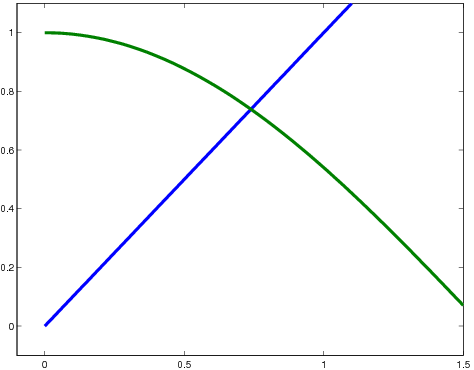
\includegraphics[height=5cm]{figures/fixpunkt}
\end{center}
Voraussetzung: Abbildung kontrahierend 
\[
\abs{f(x)-f(y)} \leq C \abs{x-y},\, C < 1\,  \forall  x,y \in  I
\]
% offenes Intervall I

\end{frame}
%
% - Folie
%
\begin{frame}[fragile]\frametitle{Fixpunkt-Iteration}
Fixpunkt-Iteration 
\[ x_{k+1}=cos(x_k) \]
bei geeignetem Startwert $x_0$.  \\
\centering{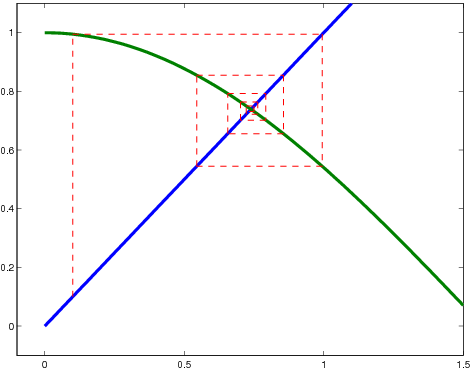
\includegraphics[height=5cm]{figures/fixpunkt1}}\\
(Funktioniert wenn die Abbildung kontrahierend ist)
\end{frame}

%
% - Folie
%
\begin{frame}[fragile]\frametitle{Fixpunkt-Iteration - Implementation}
\begin{lstlisting}
% Plot 1
x = linspace(0,1.5,50);
y = cos(x);
plot(x,x,x,y,'LineWidth',3),
axis([-0.1 1.5 -0.1 1.1]);
hold on;
pause; % stoppt bis eine Taste gedrückt wird
z(1) = 0.1; % Anfangswert
it_max = 10; % Iterationsschritte 
for i = 1:it_max
    z(i+1) = cos(z(i));
    plot([z(i) z(i)], [z(i) z(i+1)],'r--','LineWidth',1);
    pause;
    plot([z(i) z(i+1)],[z(i+1) z(i+1)],'r--','LineWidth',1);
    hold on;
    pause; % stoppt bis eine Taste gedrückt wird
end;
\end{lstlisting}
\end{frame}
%
% - Folie
%
\begin{frame}[fragile]\frametitle{Einige Grafikbefehle}
\begin{itemize}
\item \alert{ \mcode{figure}} \\
startet ein Grafik-Fenster.
\item \alert{ \mcode{hold on}}\\
 alle Grafiken in einem Fenster werden \"ubereinander gezeichnet. 
\item \alert{ \mcode{hold off}} (Standard)\\
 bestehende Grafik wird gel\"oscht und durch die neue Grafik ersetzt.
\end{itemize}
\end{frame}
\begin{frame}[fragile]\frametitle{Vandermonde-Matrix I}
Berechne zu einem gegebenen Vektor
  $x=(x_1, \dots ,x_n)$ die Vandermonde-Matrix
{ \[ V:= \left(\begin{array}{ccccc} 
1 & x_1 & x_1^2 & \hdots & x_1^{n-1}\\
1 & x_2 & x_2^2 & \hdots & x_2^{n-1}\\
\vdots & \vdots & \vdots & \vdots & \vdots\\
1 & x_n & x_n^2 & \hdots & x_n^{n-1}\\
\end{array} \right).  \]}
\end{frame}
%
%
%
\begin{frame}[fragile]\frametitle{Vandermonde-Matrix II}
\lstinputlisting{vandermonde2.m}
\end{frame}



\subsection{Bedingungen}
%
%
%
\begin{frame}[fragile]\frametitle{Quadratische Gleichung}
\alert{ \[  \left\{ \begin{array}{l} \mbox{Suche }  x \in \mathbb{R},
 \mbox{ so dass } \\
 x^2+px +q =0  \end{array} \right. \]}
Fallunterscheidung für $d:=\frac{p^2}{4} -q$:
\begin{description}
\item [Fall a)]: \alert{ $d>0$} \quad 2 Lösungen: $x=-\frac{p}{2} \pm \sqrt{d}$ \\
\item [Fall b)]: \alert{ $d=0$} \quad 1 Lösung: $x=-\frac{p}{2}$\\
\item [Fall c)]: \alert{ $d<0$} \quad keine Lösung
\end{description}
\end{frame} 
%
%
%
\begin{frame}[fragile]\frametitle{Implementierung}
\begin{lstlisting}
function [anz_loesungen, loesungen]=quad_gl(p,q)
%----------------------------------------------------
% quad_gl berechnet die Loesungen der quadratischen   
%         Gleichung x^2 + px + q =0
%           INPUT:   Skalare   p
%                              q
%                 
%           OUTPUT: anz_loesungen   Anzahl der Loesungen
%                   loesungen       Vektor der Loesungen
%
%  Gerd Rapin      8.11.2003
%------------------------------------------------------
d=p^2/4-q; % Diskriminante


\end{lstlisting}
\end{frame}
%
%
%
\begin{frame}[fragile]\frametitle{Implementierung II}
\begin{lstlisting}
% 2 Loesungen
if d>0 
    anz_loesungen=2;
    loesungen=[-p/2-sqrt(d) -p/2+sqrt(d)];
end

% 1 Loesung
if d==0 
    anz_loesungen=1;
    loesungen=[-p/2];
end

% 0 Loesungen
if d<0 
    anz_loesungen=0;
    loesungen=[];
end
\end{lstlisting}
\end{frame}

%
%
%
\begin{frame}[fragile]\frametitle{Logische Operationen}
\begin{itemize}
\item logische Variablen (Datentyp ist \alert{logical}). 
\item Variablen dieses Typs sind entweder \mcode{TRUE} (1) oder
  \mcode{FALSE} (0).
\item Numerische Werte ungleich $0$ werden als \mcode{TRUE} gewertet.
\end{itemize}
\begin{lstlisting}
a = (1<2)
\end{lstlisting}
\begin{matlab}
a = 1 
\end{matlab}
\begin{lstlisting}
b = ([ 1 2 3 ] < [ 2 2 2 ]) 
\end{lstlisting}
\begin{matlab}
b =   1     0     0 
\end{matlab}
\begin{lstlisting}
whos 
\end{lstlisting}
\begin{matlab}
  Name Size Bytes  Class
  a     1x1  1  logical array
  b     1x3  3  logical array 
\end{matlab}
\end{frame}
%
%
%
\begin{frame}[fragile]\frametitle{Vergleichs-Operatoren}
\begin{lstlisting} 
a=[1 1 1], b=[0 1 2] 
\end{lstlisting}
\begin{center}
\begin{tabular}{cll}
Operation & Bedeutung & Ergebnis\\
\hline
\mcode{a == b} & gleich &   \mcode{0     1     0}\\
\mcode{a \~= b} & ungleich & \mcode{1     0     1}\\
\mcode{a < b} & kleiner & \mcode{0     0     1}\\
\mcode{a > b} & größer & \mcode{1     0     0}\\
\mcode{a <= b} & kleiner oder gleich & \mcode{0     1     1}\\
\mcode{a >= b} & größer oder gleich & \mcode{1     1     0}\\
\end{tabular}
\end{center}
\alert{Bem:} \alert{ 1 = wahre Aussage, 0 = falsche Aussage}\\
\alert{Bem:} Komponentenweise Vergleiche sind auch für Matrizen
gleicher Größe möglich! 
\end{frame}
%
%
%
\begin{frame}[fragile]\frametitle{Logische Operatoren}
\begin{center}
\begin{tabular}{|c|l||c|l|}
\hline
\mcode{\&} & logisches und & \mcode{\~} & logisches nicht \\
\mcode{|} & logisches oder & \mcode{xor} & exklusives oder\\
\hline
\end{tabular}
\end{center}
Beispiele:\\
\begin{lstlisting} 
x=[-1 1 1]; y=[1 2 -3];
\end{lstlisting}
\vspace*{0.5cm}
\begin{minipage}{5cm}
\begin{lstlisting}
>> (x>0) & (y>0)
ans =
     0     1     0
\end{lstlisting}
\vspace*{0.5cm}
\begin{lstlisting}
>> (x>0) | (y>0)
ans =
     1     1     1
\end{lstlisting}
\end{minipage} \hfill
\begin{minipage}{5cm}
\begin{lstlisting}
>> ~( (x>0) & (y>0))
ans =
     1     0     1
\end{lstlisting}
\vspace*{0.5cm}
\begin{lstlisting}
>> xor(x>0,y>0)
ans =
     1     0     1
\end{lstlisting}
\end{minipage}
\end{frame}
%
%
%
\begin{frame}[fragile]\frametitle{Bedingung}
\begin{columns}[t,onlytextwidth]
 \column{0.45\textwidth}
Einfache Bedingung
\begin{lstlisting}
if  <Ausdruck>
   <Befehle>
end
\end{lstlisting}
 \column{0.45\textwidth}
Bed. mit Alternative
\begin{lstlisting}
if  <Ausdruck>
   <Befehle>
else
   <Befehle>
end
\end{lstlisting}
\end{columns}

Die Befehle zwischen \mcode{if} und \mcode{end} werden ausgeführt, wenn
der \textit{Ausdruck} wahr (\mcode{TRUE}) ist. 
Andernfalls werden (soweit vorhanden) die
Befehle zwischen \mcode{else} und \mcode{end} ausgeführt.

\textit{Ausdruck} ist wahr, wenn   alle Einträge von \textit{Ausdruck} ungleich $0$ sind.
\end{frame}
%
%
%
\begin{frame}[fragile]\frametitle{While-Schleifen}
\begin{lstlisting}
while <Ausdruck>
   <Befehle>
end
\end{lstlisting}
Die Befehle werden wiederholt,  so lange die Bedingung {\it Ausdruck}
wahr ist.  {\it Ausdruck} ist wahr, wenn   alle Einträge von {\it
  Ausdruck} ungleich $0$ sind. \\[1cm] 

\textbf{Beispiel:} Berechne \alert{ $\sum_{i=1}^{1000} \frac{1}{i}$}.
\begin{lstlisting}
n = 1000; sum = 0; i = 1; 
while (i <= n) 
  sum = sum+(1/i); 
  i = i+1;  
end
sum
\end{lstlisting}

\end{frame}
%
%
%
\begin{frame}[fragile]\frametitle{Größter gemeins. Teiler (ggT)}
Berechnung des ggT von natürlichen Zahlen $a$ und $b$ mit Hilfe des
euklidischen Algorithmus\\[1cm]

\alert{Idee:} Es gilt \alert{ $ggT(a,b)=ggT(a,b-a)$} für $a<b$.\\[1cm]

\alert{Algorithmus:} \\
Wiederhole,  bis $a=b$
\begin{itemize}
\item Ist $a>b$, so $a=a-b$.
\item Ist $a<b$, so $b=b-a$ 
\end{itemize}
\end{frame}

\begin{frame}[fragile]\frametitle{Implementierung}
\lstinputlisting{ggt.m}
\end{frame}
%
%
%
\begin{frame}[fragile]\frametitle{\textit{break}}
\begin{itemize}
\item  Der Befehl \mcode{break} verläßt die \mcode{while} oder
  \mcode{for}-Schleife.
\begin{matlabin}
x=1;
while 1
  xmin=x;
  x=x/2;
  if x==0
    break
  end
end
xmin
\end{matlabin}
\begin{matlab}
xmin = 4.9407e-324
\end{matlab} 

\end{itemize}
\end{frame}

\begin{frame}[fragile]\frametitle{\textit{continue}}
\begin{itemize}
 \item  Durch \mcode{continue} springt man sofort in die
  nächste Iteration der Schleife, ohne die restlichen Befehle zu
  durchlaufen.
\begin{matlabin}
for i=1:10
  if i<5
    continue
  end
  x(i)=i;
end
x
\end{matlabin}
\begin{matlab}
x =  0  0  0  0  5  6  7  8  9  10
\end{matlab}
 
\end{itemize}
\end{frame}



\subsection{Allgemeines}
%
% Folie
%
\begin{frame}[fragile]\frametitle{Operator Rangfolge}
\begin{tabular}{|cp{10cm}|}
\hline
Level & Operator\\
\hline
1 &   Exponent (\mcode{^}, \mcode{.^}), \mcode{transpose}\\
2 & logische Verneinung (\mcode{\~})\\
3 & Multiplikation (*,.*), Division (\mcode{/},\mcode{./},\mcode{\\}, \mcode{.\\})\\
4 & Addition (+), Subtraktion (-)\\
5 & Doppelpunktoperator (:)\\
6 & Vergleichsoperatoren (\mcode{<},\mcode{>},\mcode{<=},\mcode{>=},\mcode{==},\mcode{\~=})\\ 
7 & Logisches und (\mcode{\&})\\
8 & Logisches oder (\mcode{|})\\
\hline
\end{tabular}\\[0.5cm]
{\scriptsize Bei gleicher Rangfolge wertet MATLAB von links nach rechts
  aus. \\
Die Rangfolge kann durch Klammersetzung geändert werden.}

\end{frame}


%
% Slide
%
\begin{frame}[fragile]\frametitle{Warnung}
\begin{center}
\alert{ Wiederholte Anwendung von Script-Files kann zu Fehlern führen!}\\[0.5cm]
\end{center}
\begin{columns}[t]
 \column{0.4\textwidth}
\alert{Programm}
\begin{lstlisting}[basicstyle=\scriptsize]
% plotte_sin.m

disp(['Plot der Sinus'...
  'Funktion auf [0,10]']);
n = input(['Plot an '...
   'wievielen Punkten?']);
x = linspace(0,10,n);
for i=1:n
y(i) = sin(x(i));
end; 
plot(x,y);
\end{lstlisting}
\column{0.5\textwidth}
\alert{ Aufruf}
\begin{lstlisting}[basicstyle=\scriptsize]
>> plotte_sin
Plot der Sinus Funktion auf [0,10]
Plot an wievielen Punkten?20
>> plotte_sin
Plot der Sinus Funktion auf [0,10]
Plot an wievielen Punkten?10
??? Error using ==> plot
Vectors must be the same lengths.

Error in ==> plotte_sin.m
On line 9  ==> plot(x,y);
\end{lstlisting}
\end{columns}
\end{frame}
%
% Slide
%
\begin{frame}[fragile]\frametitle{globale Variablen}
Mittels des Befehls \alert{ \mcode{global}} können Variablen des
globalen Workspace auch für Funktionen manipulierbar gemacht werden.
\bigskip
\begin{columns}[t]
 \column{0.45\textwidth}
\alert{ Funktion}
\begin{lstlisting}
function f=myfun(x)
% myfun.m
% f(x)=x^alpha sin(1/x)

global alpha
f=x.^alpha.*sin(1./x);
\end{lstlisting}
 \column{0.45\textwidth}
\alert{ Plotten}
\begin{lstlisting}
% plot_myfun
global alpha
alpha_w=[0.4 0. 6 1 1.5 2];
for i = 1:length(alpha_w)
    alpha = alpha_w(i);
    fplot(@myfun,[0.1,1])
    hold on;
end
hold off;
\end{lstlisting}
\end{columns}
\end{frame}
%
% Slide
%
\begin{frame}[fragile]\frametitle{Ein Guter Stil}
\begin{itemize}
\item Alle Programme sollten zu Beginn einen Kommentar enthalten, in
  dem beschrieben wird, was das Programm macht. Insbesondere sollten
  die Eingabe- und Ausgabevariablen  genau beschrieben
  werden. 
\item Vor und nach logischen Operatoren und $=$ sollte ein Leerzeichen
  gesetzt werden.
\item Man sollte pro Zeile nur einen Befehl verwenden.
\item Befehle in  Strukturen, wie  \mcode{if}, \mcode{for}
  oder \mcode{while}, sollten eingerückt werden. 
%\item Variablen Namen für Matrizen sollten mit einem Großbuchstaben
 % beginnen. 
\end{itemize}
\end{frame}
%
% Slide
%
\begin{frame}[fragile]\frametitle{Ein Guter Stil}
\begin{itemize}
\item Die Namen der Variablen sollten, soweit möglich, selbsterklärend
  sein.
\item Verfasst man umfangreiche Programme, so sollten M-Funktionen, die
  eine logische Einheit bilden in einem separaten Unterverzeichnis
  gespeichert sein. Die Verzeichnisse können durch \mcode{addpath}
  eingebunden werden. 
\item Potenzielle Fehler sollten, soweit möglich, aufgefangen
  werden. Speziell sollten die Eingabeparameter der Funktionen
  geprüft werden. 
\end{itemize}
\end{frame}


\section{Datenstrukturen}
%
%
%
\begin{frame}[fragile]\frametitle{Datentypen}
\begin{itemize}
\item \alert{Datentypen} werden bestimmt durch ihre Eigenschaften.
\item Einzelne Elemente eines Datentyps werden \alert{Objekte} genannt. 
\item Ein \alert{Objekt} besteht meist aus drei Teilen: \alert{Bezeichner}, \alert{Referenzen} 
und \alert{Werte} des Objekts.  
\item \alert{Variablen} sind Datenobjekte deren Werte w\"ahrend eines
Programmablaufs ver\"andert werden k\"onnen. 
\end{itemize}
\end{frame}
%
%
%
\begin{frame}[fragile]\frametitle{Datentypen in MATLAB}
\begin{itemize}
\item Alle Variablen sind Felder (Array). Ein Skalar ist eine $1 \times
1$-Matrix. 
\item Zuweisung des Datentyps {\it implizit}. 
\item Den Datentyp eines Objekts $a$ kann durch den Befehl \mcode{class(a)} bestimmt werden.
\end{itemize}
\end{frame}
%
%
%
\begin{frame}[fragile]\frametitle{Datentypen in MATLAB}
\begin{itemize}
\item Gleitkommazahlen (Komplexe Zahlen)
\item Characters und Strings
\item Strukturen
\item Cell Arrays
\item Funktionen
\item Sparse Matrizen
\item Integer-Zahlen
\item Logische Ausdr\"ucke
\end{itemize}
\end{frame}

\subsection{Zahlen}
%
% Folie
%
\begin{frame}[fragile]\frametitle{Gleitkommazahlen / Maschinengenauigkeit}
\begin{itemize}
\item Standard-Datentyp ist ein Array von Gleitkommazahlen (\mcode{double}).
\item Abstand von $1$ zur nächsten Gleitkommazahl: $\epsilon
  = 2^{-52} \sim 2.2\cdot10^{-16}$ (vgl. \mcode{eps})
\item Sei $x \in \mathbb{R}$ eine reelle Zahl und $\tilde x$ die
  Darstellung in MATLAB. Dann gilt für den Rundungsfehler \\[-0.5cm]
\[ \frac{|x - \tilde x|}{|x|}\leq \frac{1}{2} \epsilon .\]
\item Die größte bzw. kleinste in MATLAB darstellbare positive Zahl
  ist in
\mcode{realmin} bzw. \mcode{realmax} gespeichert. 
\end{itemize}
\end{frame}
%
% Folie
%
\begin{frame}[fragile]\frametitle{Ausnahmen}
\begin{itemize}
\item Ist eine Zahl größer als \mcode{realmax}, so meldet MATLAB einen
  'Overflow' und gibt als Ergebnis \mcode{Inf} zurück.
\begin{lstlisting}
realmax*1.1
\end{lstlisting}
\begin{matlab}
 ans =   Inf
\end{matlab}

\item Bei Operationen wie $0/0$  oder $\infty / \infty$, erhält man als Ergebnis
  \mcode{NaN} ({\it Not a Number}).
\begin{lstlisting}
0/0 
\end{lstlisting}
\begin{matlab}
Warning: Divide by zero.
ans =   NaN 
\end{matlab}

\end{itemize}
\end{frame}
%
% Folie
%
\begin{frame}[fragile]\frametitle{Umgang mit NaN und       Inf  }
\begin{itemize}
\item Mit Hilfe von \alert{ \mcode{isinf}} und \alert{ \mcode{isnan}} kann auf
$\infty$ bzw. NaN getestet werden.
 \begin{lstlisting}
isnan(0/0), isinf(1.2*realmax)
\end{lstlisting}
\begin{matlab}
ans =   1  ans =   1
\end{matlab}
\item Test auf NaN durch $==$ ist nicht m\"oglich
\begin{lstlisting}
0/0 == NaN
\end{lstlisting}
\begin{matlab}
ans =     0
\end{matlab}
\item Bei Inf ist der Test durch $==$  m\"oglich!
\begin{lstlisting}
(1.2*realmax)==Inf
\end{lstlisting}
\begin{matlab}
ans =     1
\end{matlab}
\end{itemize}
\end{frame}
%
% Folie
%
\begin{frame}[fragile]\frametitle{Single}
\begin{itemize}
\item \"Ahnlich wie in C gibt es den Datentyp \mcode{single}. Es ist eine
Darstellung in geringerer Genauigkeit. 
\item Durch den Befehl \alert{ \mcode{single()}} wird eine \mcode{double}-Zahl in
eine \mcode{single}-Zahl konvertiert. 
\item Arithmetische Operationen mit \mcode{double}- und \mcode{single}-Objekten
ergeben  \mcode{single}-Objekte.
\end{itemize}
\end{frame}
%
% Folie
%
\begin{frame}[fragile]\frametitle{Single}
\begin{lstlisting}
a = sqrt(2); b = single(a);
c = a+b; d = a-b
\end{lstlisting}
\begin{matlab}
d =
  2.4203e-08
\end{matlab}
\begin{lstlisting}
whos
\end{lstlisting}
\begin{matlab}
  Name   Size     Bytes  Class    
  a      1x1        8  double              
  b      1x1        4  single              
  c      1x1        4  single              
  d      1x1        4  single  
\end{matlab}
\begin{lstlisting}
[realmax, single(realmax)], realmax
\end{lstlisting}
\begin{matlab}
ans =
   Inf   Inf
ans =
  1.7977e+308
\end{matlab}
\end{frame}

%
% Folie
%
\begin{frame}[fragile]\frametitle{Darstellungsformate am Beispiel $1/7$}
\begin{tabular}{ll}
\alert{ \mcode{format short}} &  0.1429 \\
\alert{ \mcode{format short e} }& 1.4286e-01\\
\alert{ \mcode{format short g} }&0.14286\\
\alert{ \mcode{format long} }& 0.14285714285714\\
\alert{ \mcode{format long g} }& 0.142857142857143\\
\alert{ \mcode{format long e} }& 1.428571428571428e-01\\
\end{tabular}

Das Default-Format ist \mcode{short}. 
\end{frame}


\begin{frame}[fragile]{Beispiel - Berechnung von $e$}
Approximation der Exponentialfunktion durch eine Taylor-Reihe
\begin{equation*}
 P_n(x) = \sum_{j=0}^n\frac{x^j}{j!} 
\end{equation*}

\lstinputlisting{calcexp.m}
\end{frame}

\begin{frame}[fragile]{Berechnung von $e$ - Figure}
\begin{center}
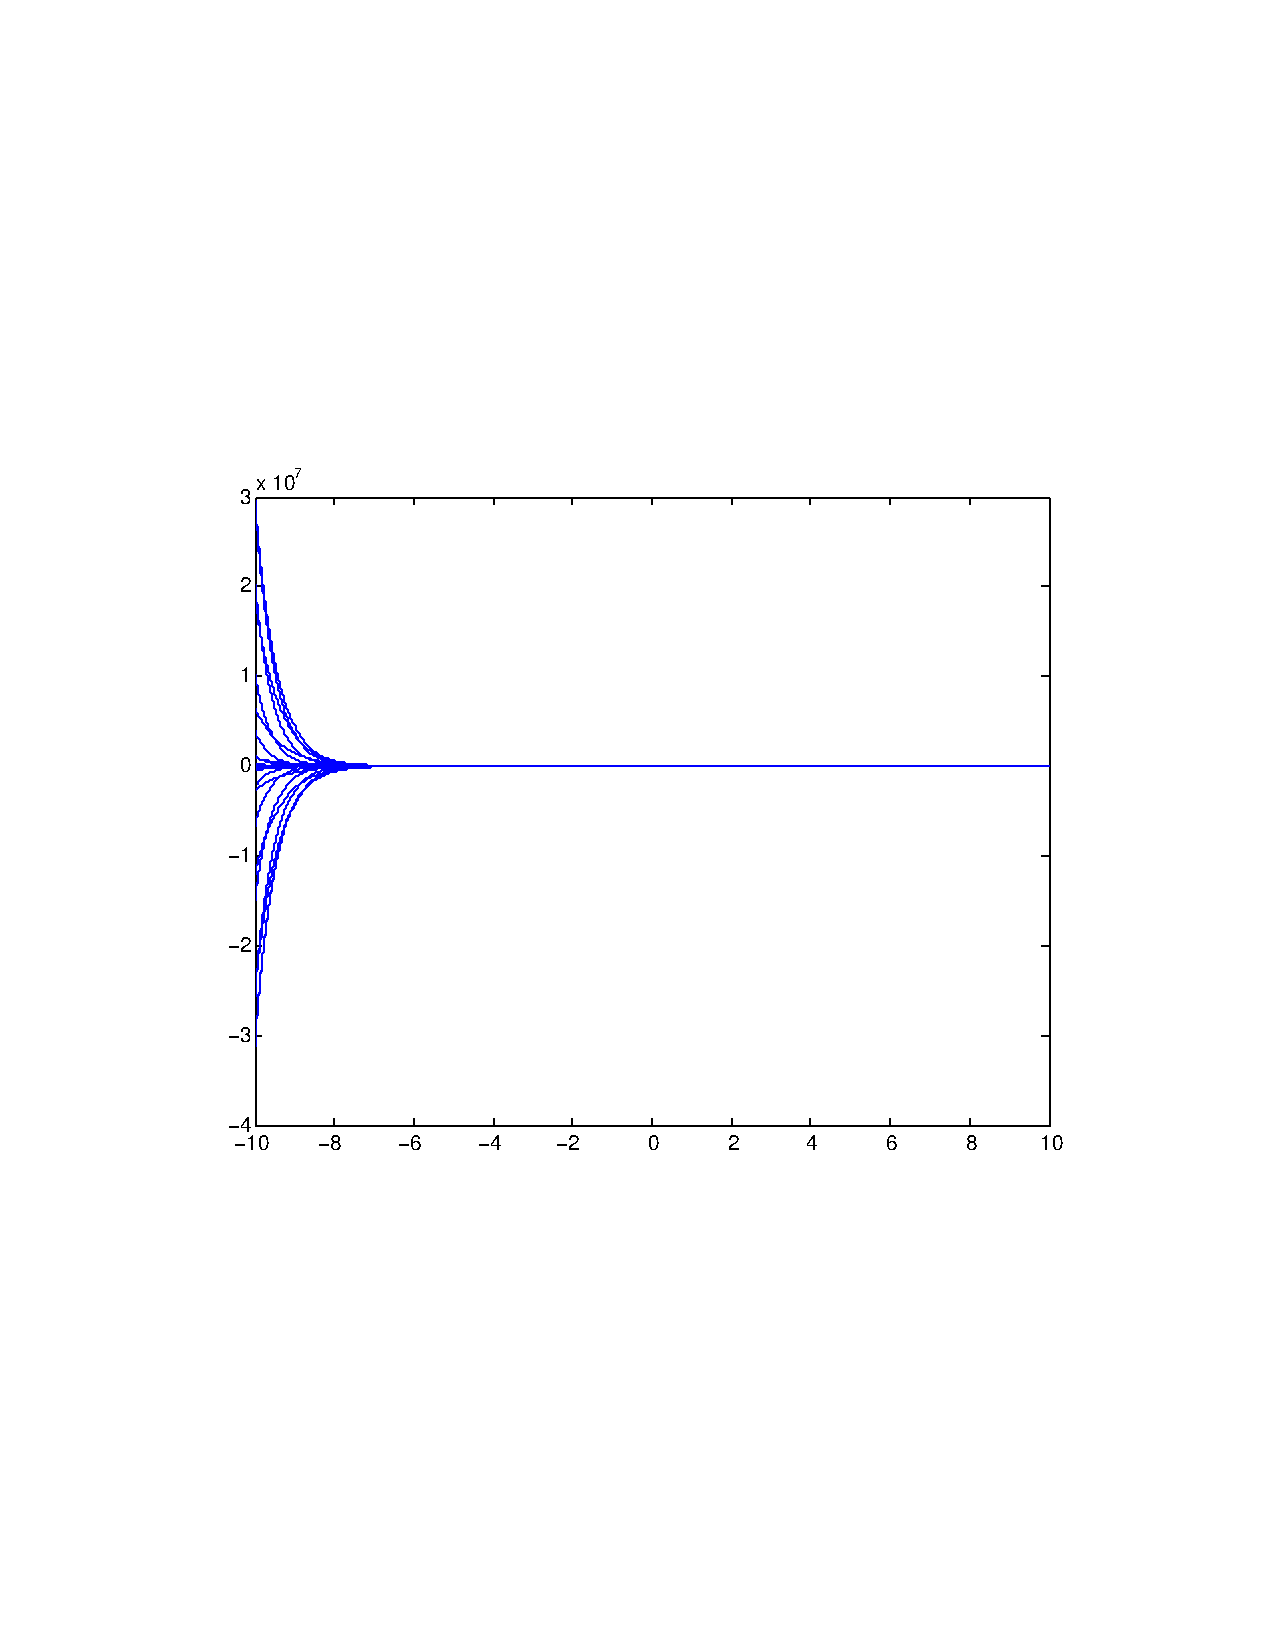
\includegraphics[height=7cm]{figures/calcexp}
\end{center}
\end{frame}

\begin{frame}[fragile]{Auslöschung}
\lstinputlisting{ausloeschung.m}
\begin{matlab}
x = 0.344152
xwahr = 0.3441520344152
relfx = 9.99999900671778e-08
y = 0.344135
z = 1.69999999999892e-05
zwahr = 1.70344152000124e-05
relfz = 0.00202033352005498
\end{matlab}

\end{frame}



%
% Folie
%
\begin{frame}[fragile]\frametitle{Komplexe Zahlen}
Komplexe Zahlen $z \in \mathbb{C}$ haben die Form
\[ z = x +iy, \quad x,y \in \mathbb{R} \]
mit $i=\sqrt{-1}$. 
\begin{itemize}
\item $\sqrt{-1}$ ist in MATLAB vordefiniert in den Variablen $i$,$j$.
\item Durch \mcode{complex(x,y)}  kann aus $x,y \in
  \mathbb{R}$ die komplexe Zahl $x + iy$ erzeugt werden.
\item Für $z=x+iy \in \mathbb{C}$ erhält man den Realteil mit
  $real(z)$ und den Imaginärteil durch $imag(z)$. 
\end{itemize} 
\end{frame}
\begin{frame}[fragile]\frametitle{Polarkoordinaten}
\alert{ \[ z \in \mathbb{C}, \quad z=re^{i \varphi}=r(\cos \varphi + i \sin
  \varphi) \]}
\begin{itemize}
\item \mcode{abs(z)} ergibt den Betrag $r$ von $z$.
\item $\varphi$ erhält man durch \mcode{angle(z)}.
\item grafische Darst.:  \mcode{compass(z)} ($z=3+3i$). \\
 \centering{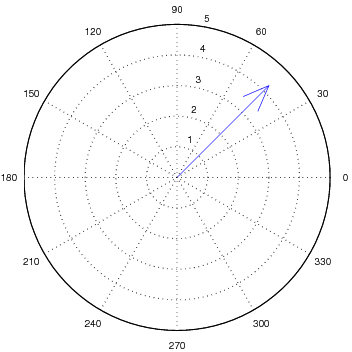
\includegraphics[width=0.3\textwidth]{../figures/kompass}}\\ 
\end{itemize}
\end{frame}

%
% Folie
%
\begin{frame}[fragile]\frametitle{Integer}
\begin{itemize}
\item In diesen Datentypen werden ganze bzw. nat\"urliche Zahlen gepeichert.  
\item Zur effizienten Speicherung gibt es die Datentypen \mcode{int8},
\mcode{uint8}, \mcode{int16}, \mcode{uint16}, \mcode{uint16}, \mcode{int32},
\mcode{uint32}, \mcode{int64}, \mcode{uint64}. 
\item In den Datentypen, die mit \mcode{u} beginnen, werden nat\"urliche Zahlen
gespeichert, sonst ganze Zahlen.
\item Die abschlie{\ss}ende Zahl gibt den Speicherbedarf an. \mcode{uint8}
ben\"otigt z.B. $8$-Bit. (Wertebereich $0 \dots 2^8-1$).
\end{itemize}
\end{frame}
%
% Folie
%
\begin{frame}[fragile]\frametitle{Integer}
\begin{lstlisting}
a = int8(20); b = int16(20); c = int8(20);
a*c, a*b
\end{lstlisting}
\begin{matlab}
ans =  127
??? Error using ==> mtimes
Integers can only be combined with integers
of the same class, or scalar doubles.
\end{matlab}
\begin{lstlisting}
a+0.2
\end{lstlisting}
\begin{matlab}
ans =   20
\end{matlab}
\begin{lstlisting}
a+0.5
\end{lstlisting}
\begin{matlab}
ans =   21
\end{matlab}
\begin{lstlisting}
a*1.54
\end{lstlisting}
\begin{matlab}
ans =   31
\end{matlab}
\end{frame}
%
%
%

\subsection{Container}
%
% Folie
%
\begin{frame}[fragile]\frametitle{Structures}
\alert{Structures:}\\
Strukturen sind eine Möglichkeit verschiedene Objekte in einer
Datenstruktur zu bündeln.\\[1cm]

\alert{Beispiel:} komplexe Zahlen
\begin{lstlisting}
komp_Zahl.real=1;
komp_Zahl.imag=1;
komp_Zahl
\end{lstlisting}
\begin{matlab}
komp_Zahl = 

    real: 1
    imag: 1
\end{matlab}
\end{frame}
%
% Folie
%
\begin{frame}[fragile]\frametitle{Structures II}
\begin{itemize}
\item Alternativ können Strukturen durch
\begin{lstlisting}
struktur = struct('Feld1',<Wert1>,'Feld2',<Wert2>,..)
\end{lstlisting}
definiert werden.
\item Ein Feld einer Struktur \mcode{struktur} kann durch 
\begin{lstlisting}
struc2 = rmfield( <struktur> ,'Feld')
\end{lstlisting}
gel\"oscht werden. 
\end{itemize}
\end{frame}
%
% Folie
%
\begin{frame}[fragile]\frametitle{Cell Arrays}
\alert{Cell Arrays:} \\
Cell Arrays sind spezielle Matrizen, deren  Einträge aus unterschiedlichen
Datentypen bestehen können. Erzeugt
werden sie durch geschweifte Klammern.\\
\begin{lstlisting}
C = { 1:10, hilb(4);...
       'Hilbert Matrix', pi}
\end{lstlisting} 
\begin{matlab}
C = 
       [1x10 double]    [4x4 double]
    'Hilbert Matrix'    [    3.1416]
\end{matlab} 
\end{frame}
%
% Folie
%
\begin{frame}[fragile]\frametitle{Befehle für Cell Arrays}
\begin{itemize}
\item Zugriff auf Cell-Arrays:\\ 
\begin{columns}[c]
\column{0.45\textwidth}
\begin{lstlisting} 
C{2,1}
\end{lstlisting}
\begin{matlab}
ans =
Hilbert Matrix
\end{matlab}
\column{0.45\textwidth}
\begin{lstlisting}
C{1,2}(2,3)
\end{lstlisting}
\begin{matlab}
ans =
    0.2500
\end{matlab}
\end{columns}
\item Durch \mcode{celldisp(C)} wird der Inhalt von $C$ dargestellt.
%\item \mcode{struct2cell} bzw. \mcode{num2cell} erzeugt ein Cell Array
%  aus einer Struktur bzw. einer normalen Matrix.
\item \mcode{cellplot(C)} stellt $C$ grafisch dar.
\end{itemize}
\end{frame}

\subsection{Chars und Strings}
%
% Folie
%
\begin{frame}[fragile]\frametitle{Characters (char) - Zeichen}
\begin{itemize}
 \item Darstellung durch Integer
 \item Die Werte zwischen 0 und 128 entsprechen den ASCII Werten. 
\item 2 Bytes Speicherbedarf $\Rightarrow$ Zahl zwischen 0 und $2^{16}-1$ 
\end{itemize}

\begin{lstlisting}
s='d'
\end{lstlisting}
\begin{matlab}
s = d
\end{matlab}
\begin{lstlisting}
s1=double(s)
\end{lstlisting}
\begin{matlab}
s1 =  100
\end{matlab}
\begin{lstlisting}
s2=char(100)
\end{lstlisting}
\begin{matlab}
s2 = d
\end{matlab}
\end{frame}
%
% Folie
%
\begin{frame}[fragile]\frametitle{Strings - Vektor von Zeichen}
Die Zeichen werden wiederum durch die ASCII Werte dargestellt. 
\begin{lstlisting}
s='AB6de*'
\end{lstlisting}  
\begin{matlab}
s =
AB6de*
\end{matlab}
\begin{lstlisting}
sd=double(s)
\end{lstlisting}  
\begin{matlab}
sd =
    65    66    54   100   101    42
\end{matlab}
\begin{lstlisting}
s2=char(sd)
\end{lstlisting}  
\begin{matlab}
s2 =
AB6de*
\end{matlab}
\end{frame}

%
% Folie
%
\begin{frame}[fragile]\frametitle{Befehle für Strings}
\begin{itemize}
\item Durch \mcode{strcat} werden Strings verbunden, z.B. 
\begin{lstlisting}
strcat('Hello',' world') 
\end{lstlisting}
\begin{matlab}
ans = Hello world 
\end{matlab}
\item \alert{\mcode{num2str(x,n)}} konvertiert $x$ in einen String mit $n$
  signifikanten Stellen. (Default: $n=4$)
\item \alert{\mcode{int2str(x)}} rundet $x$ und konvertiert es in einen String.
\item \alert{\mcode{strcmp(s,t)}} vergleicht die Strings $s$ und $t$. 
\item Durch \alert{\mcode{help strfun}} erhält man eine Liste aller Befehle im
  Zusammenhang mit Strings.
\end{itemize}
\end{frame}



\end{document}